\setcounter{subsection}{0}
\section{DESARROLLO DE LA SOLUCIÓN}

% Inserta una captura si el archivo existe en figures/capturas/; si no, deja un recuadro visible.
\newcommand{\capturaopcional}[4]{%
  \begin{figure}[H]\centering
  \IfFileExists{figures/capturas/#1}{\includegraphics[width=#2\textwidth]{capturas/#1}}{\fbox{\parbox{0.8\textwidth}{\centering\vspace{1.5cm}\textbf{[Insertar captura: #1]}\vspace{1.5cm}}}}
  \caption{#3}\label{#4}\end{figure}}

Este capítulo cuenta cómo se construyó la solución, la relaciona con la metodología de la propuesta y muestra el producto final.

\subsection{Proceso de desarrollo}

\textbf{Organización del equipo y esfuerzo.} El equipo fue de cuatro estudiantes con la dirección del ingeniero Calderón; no hubo \textit{Product Owner} externo, por lo que el equipo ordenó el \textit{backlog} por prioridad. La línea base de esfuerzo fue de 600 horas-persona, a las que se sumaron 120 de la extensión de la versión 2.0, para un total de 720. Se planificaron 10 semanas efectivas dentro de un semestre de 16 como colchón de riesgo. La figura~\ref{fig:wbs} muestra la estructura de desglose del trabajo y la figura~\ref{fig:gantt} el cronograma de la línea base.

\begin{figure}[H]
\centering
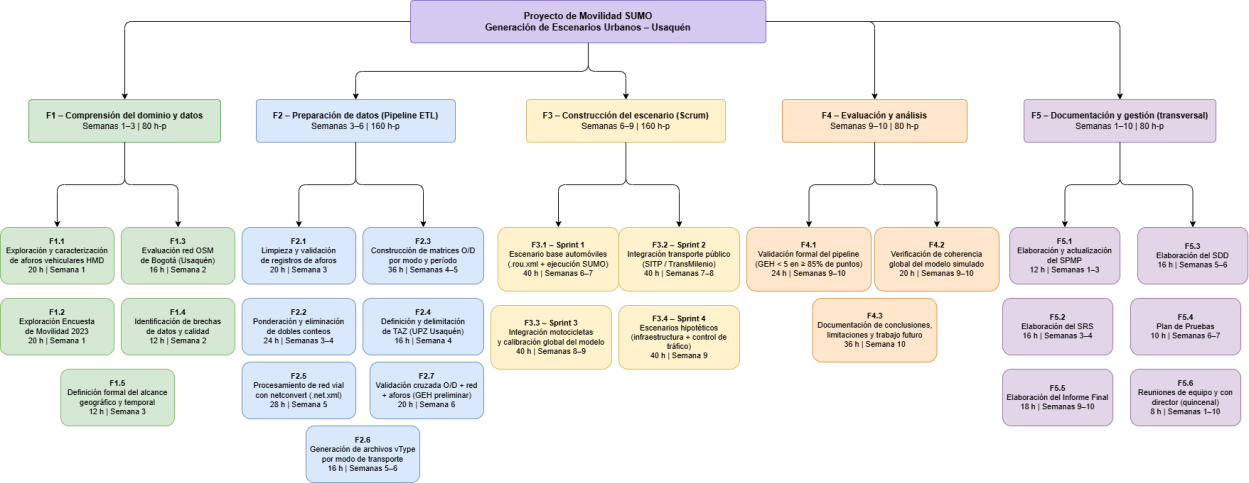
\includegraphics[width=\textwidth]{fig08-wbs-linea-base.png}
\caption{Estructura de desglose del trabajo (línea base).}
\label{fig:wbs}
\end{figure}

\begin{figure}[H]
\centering
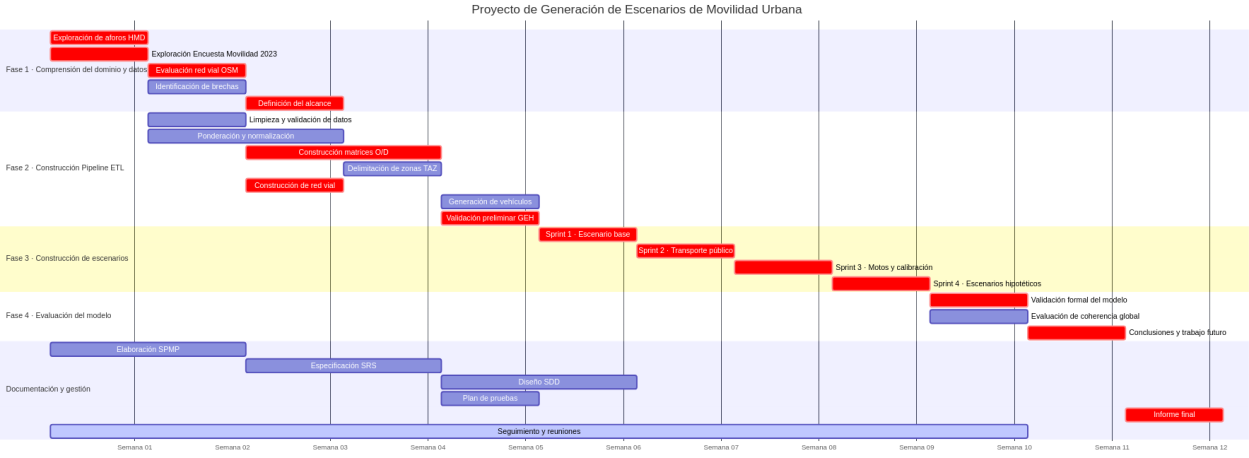
\includegraphics[width=\textwidth]{fig09-gantt-linea-base.png}
\caption{Cronograma de la línea base.}
\label{fig:gantt}
\end{figure}

\textbf{Fase 1: comprensión del dominio y de los datos (CRISP-DM).}
\label{sec:fase1}
Se exploraron tres fuentes: los aforos vehiculares de hora de máxima demanda (HMD), la Encuesta de Movilidad 2023 y la red vial de OpenStreetMap. Los hallazgos principales fueron:
\begin{itemize}[noitemsep]
    \item La encuesta tiene 100.174 viajes; 9.341 tocan Usaquén y 2.648 son internos, una muestra suficiente para desagregar por modo y hora.
    \item La UTAM Paseo de los Libertadores tiene la peor cobertura muestral (44,4\,\%) y límites territoriales recientemente redefinidos; la UTAM Santa Bárbara tiene 75\,\%.
    \item Los aforos HMD son vehiculares por diseño y no cubren bien los viajes a pie; además, no traen coordenadas, solo texto libre de localización, de modo que las 336 estaciones no pudieron geocodificarse a tiempo.
    \item En la red de OSM, la cobertura de atributos es baja (velocidad máxima 23,2\,\%, carriles 27,8\,\%, nombre 41,9\,\%) y hay un área sin trazado en el Country Club.
\end{itemize}
La brecha de los aforos sin geocodificar es la causa de que la validación por GEH no pudiera completarse (sección~\ref{sec:limitaciones-resultados}). El alcance se definió como la localidad de Usaquén, con la ventana de 7:00 a 10:00.

\textbf{Fase 2: preparación de datos.} Se implementó el \textit{pipeline} ETL: extracción de la encuesta y de la red; transformación (limpieza, expansión por factores de ponderación y zonificación TAZ); y carga en archivos de SUMO. La red se procesó con \texttt{netconvert} a partir de OpenStreetMap; se incorporó elevación (\texttt{usaquen\_3d\_v2.net.xml}) para disponer de la coordenada $z$ en las salidas, y la red final tiene 28.080 \textit{edges}, 7.338 cruces de prioridad y 220 semáforos. Se definieron nueve tipos de vehículo (\texttt{vType}) para los modos del sistema.

\textbf{Fase 3: construcción del escenario (Scrum).} El trabajo se organizó en sprints de dos semanas. La definición de «terminado» de la propuesta (GEH $<5$ en 85\,\% de los puntos de conteo) se mantuvo para el escenario simulado, y para los incrementos de software se usó: pruebas automatizadas que pasan y flujo demostrado en el visor. La tabla~\ref{tab:sprints} resume lo realizado.

\begin{table}[ht]
\renewcommand{\arraystretch}{1.15}
\centering
\small
\begin{tabular}{|p{2cm}|p{9.2cm}|p{2.8cm}|}
\hline
\textbf{Sprint} & \textbf{Contenido} & \textbf{Estado} \\ \hline
1 & Escenario base con red vial y demanda de la encuesta; \textit{pipeline} TSV $\rightarrow$ viajes $\rightarrow$ rutas $\rightarrow$ simulación $\rightarrow$ GeoJSON. Corrección del orden de salida de los viajes. & Completado \\ \hline
2 y 3 & Modos adicionales y calibración. Se implementaron los nueve tipos de vehículo (bicicleta, moto, taxi, escolar, especial, informal, etc.) y los estilos de conducción; el transporte público quedó como caminata y no se calibró con aforos. & Parcial \\ \hline
4 & Escenarios hipotéticos: presets de transferencia modal, conteos por modo, semilla, estilos de conducción y cierres viales. & Completado \\ \hline
5 & Módulo web: API FastAPI, visor kepler.gl, panel de demanda, avance real y cancelación, y presets precalculados. & Completado \\ \hline
6 (v2.0) & Análisis de intersecciones: ficha de semáforos, volúmenes por acceso, edición de programas, Webster, recorte de zonas, comparación de programas, priorización. & Completado \\ \hline
7 (v2.0) & Simulador 3D comparativo: dos SUMO en lockstep, escena 3D, actor en tercera persona, HUD, riesgo, minimapa, modo manual. & Completado \\ \hline
8 (v2.0) & Reporte exportable de la comparación 3D, programa editable del semáforo propuesto y transporte público con GTFS. & Pendiente \\ \hline
\end{tabular}
\caption{Sprints y estado.}
\label{tab:sprints}
\end{table}

\textbf{Fase 4: evaluación.} Se verificaron los insumos con pruebas automáticas, se comparó la distribución de horas de salida contra la encuesta (histograma) y se documentaron las limitaciones. Los resultados están en el capítulo siguiente.

\textbf{Gestión de requerimientos, riesgos y configuración.} Los requerimientos del SRS tienen un estado (implementado, parcial, pendiente) que se actualizó al construir cada uno. Los procesos de requerimientos, riesgos, configuración y calidad se modelaron con BPMN en el SPMP. El código se versionó en Git con ramas por funcionalidad (\texttt{main}, \texttt{develop}); los datos crudos de la encuesta no se versionan y viven en un almacenamiento compartido.

\textbf{Dificultades y soluciones.}
\begin{itemize}[noitemsep]
    \item \textit{Viajes perdidos:} SUMO descartaba unos 23.000 de 24.600 viajes por llegar desordenados. Se resolvió ordenándolos por hora de salida antes de rutear.
    \item \textit{Salidas de gran tamaño:} el FCD ocupaba unos 1,4~GB. Se redujo la frecuencia de escritura, se leyó en \textit{streaming} y se comprimió el resultado a 11,7~MB.
    \item \textit{Progreso opaco:} SUMO y \texttt{duarouter} guardan su salida estándar en búfer cuando se redirige, así que no puede interpretarse. El avance de \texttt{duarouter} se obtuvo del último \texttt{depart} escrito, y el de SUMO con TraCI.
    \item \textit{Fallos de suscripción en TraCI:} suscribirse a un actor que ya salió de la red acumula errores y termina haciendo caer a SUMO 1.27. Se filtran los actores que ya salieron antes de suscribirse.
    \item \textit{Demanda escasa en zonas pequeñas:} la demanda real en una zona de 350~m era demasiado pequeña para comparar escenarios. Se completó con tráfico de fondo sintético por modo.
\end{itemize}

\subsection{Producto final}

El producto es un visor web que se conecta a la API de simulación. A continuación se describen sus funciones principales.

\textbf{Visor de simulación.} Al abrir el visor se carga la simulación de la encuesta (precalculada) y se anima sobre el mapa con una línea de tiempo; cada viaje se colorea según su modo, con una leyenda en la parte superior. El panel de demanda permite elegir uno de los cuatro presets, ajustar los conteos por modo, la escala, la semilla y el estilo de conducción, y agregar cierres viales. Si los parámetros coinciden con una simulación precalculada, el botón ofrece «Cargar simulación»; si no, «Simular» lanza una corrida con avance real por etapa y botón de cancelación, y el historial de corridas queda disponible.

\capturaopcional{visor-viajes.png}{0.95}{Visor de simulación: viajes animados por modo y panel de demanda.}{fig:visor}

\textbf{Análisis de intersecciones.} Una capa de puntos muestra los 220 semáforos de la red. Al seleccionar uno, la ficha muestra su nombre, accesos, volúmenes simulados por acceso, fases y ciclo; permite editar el programa, calcular uno con Webster y comparar programas en una zona recortada alrededor del cruce. Una segunda capa (pestaña «Semaforizar») muestra los cruces sin semáforo con su nivel de prioridad y puntaje.

\capturaopcional{ficha-interseccion.png}{0.95}{Ficha de intersección y capa de priorización.}{fig:ficha}

\textbf{Simulador 3D comparativo.} Desde un cruce candidato, el usuario fija el tráfico de fondo por modo y abre el simulador, que muestra pantalla partida: a la izquierda, el cruce sin semáforo; a la derecha, con el semáforo propuesto. La escena incluye calzadas con marcas, andenes, cebras, edificios (OSM y Microsoft, más relleno ilustrativo marcado) y un poste de semáforo por acceso. El usuario sigue en tercera persona a un vehículo o a un peatón, con cámara que evita atravesar edificios, o con vista aérea. Una barra superior y una tarjeta inferior muestran la velocidad, la acción que toma el actor (por ejemplo, acelera, frena o espera), las decisiones posibles en el siguiente cruce y el índice de riesgo calculado periódicamente con TTC, DRAC y PET. Un minimapa 2D con teselas de OpenStreetMap lo ubica en la ciudad. Hay pestañas para comparar y para ver cada lado, y un modo manual para conducir el actor con el teclado.

\capturaopcional{simulador-3d.png}{0.95}{Simulador 3D comparativo (sin semáforo | con semáforo propuesto).}{fig:sim3d}

\textbf{Operación.} Para ejecutar el sistema se instala el paquete \texttt{simulation-service} (\texttt{pip install -e .[dev]}), se levanta la API con \texttt{uvicorn api.api:app} y se ejecuta el visor con \texttt{npm run dev} (se requiere un token de Mapbox en \texttt{kepler/.env}). El \textit{pipeline} completo puede ejecutarse por línea de comandos con \texttt{python -m etl.etl}, y los presets se regeneran con \texttt{python -m etl.precalculadas}. La figura~\ref{fig:dominio} muestra el modelo del dominio del sistema.

\begin{figure}[H]
\centering
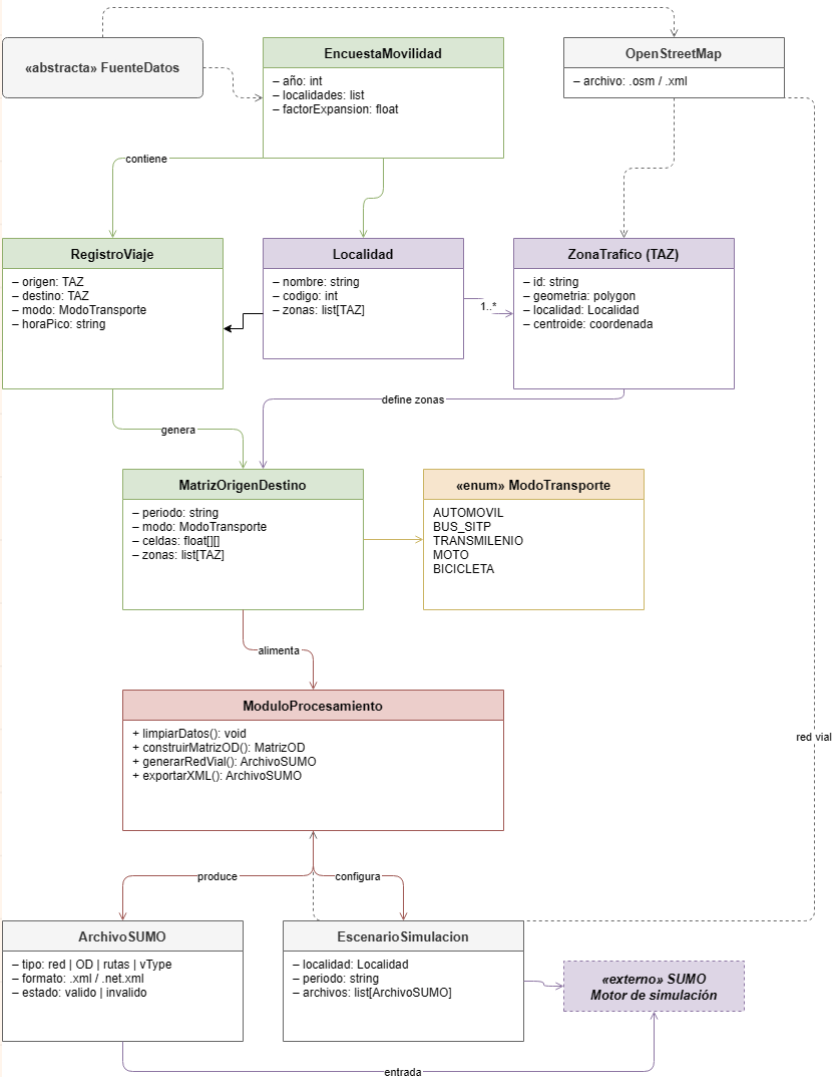
\includegraphics[height=0.42\textheight]{grafico-modelo-dominio.png}
\caption{Modelo del dominio (SRS).}
\label{fig:dominio}
\end{figure}
